\section{Direct Detection }
\label{sec:direct}
\Contributors{Kimberly Boddy, Alex Drlica-Wagner, Cora Dvorkin, Vera Gluscevic, Ethan Nadler, Lina Necib, Justin Read}

Direct detection experiments seek to directly detect interactions between particles in the Galactic dark matter halo and an experimental apparatus. In the case of WIMP dark matter, these experiments are sensitive to the scattering between dark matter particles and atomic nuclei \citep[\eg,][]{1509.08767}.
Interpreting the results of direct detection experiments in the context of dark matter necessarily relies on astrophysical measurements of the distribution of dark matter.
In addition, limitations from the kinematics and placement of direct detection experiments can limit the ranges of dark matter particle masses and cross sections that can be probed.
In this section, we describe how LSST will complement direct detection experiments by improving measurements of the local phase-space density of dark matter, and how cosmological measurements with LSST can help probe dark matter  masses and cross sections outside the range accessible to direct detection experiments.


\subsection{Local Dark Matter Distribution \Contact{Lina}}
\Contributors{Justin Read, Lina Necib}

\def\rhodm{\rho_\mathrm{\chi}}
\def\rhodmlab{\tilde{\rho}_\mathrm{\chi}}
\def\rhodmext{\rho_\mathrm{\chi,ext}}

The signal strength of dark matter scattering in direct detection experiments depends on the local dark matter density and its velocity distribution. 
For dark matter particles that scatter off atomic nuclei, the recoil rate (per unit mass, nuclear recoil energy $E$, and time) in such experiments is given by \citep[\eg,][]{1996APh.....6...87L}: 

\begin{equation}
\frac{dR}{dE} = \frac{\rhodmlab \sigma_\chi |F(E)|^2}{2 m_\chi \mu^2} \int_{v>\sqrt{m_N E/2\mu^2}}^{v_\mathrm{max}} \frac{f({\bf v},t)}{v}d^3 {\bf v} 
\label{eqn:recoilrate} 
\end{equation} 
where $\sigma_\chi$ and $m_\chi$ are the interaction cross section and mass of the dark matter particle, $|F(E)|$ is a nuclear form factor that depends on the choice of detector material, $m_N$ is the mass of the target nucleus, $\mu$ is the reduced mass of the dark matter-nucleus system, $v = |{\bf v}|$ is the speed of the dark matter particles, $f({\bf v},t)$ is the velocity distribution function of the dark matter particles, $v_\mathrm{max} = 533^{+54}_{-41}\kms$ (at 90\% confidence) is the Galactic escape speed \citep{2014AA...562A..91P}; and $\rhodmlab$ is the dark matter density within the detector. 
 
From equation \ref{eqn:recoilrate}, we can see that $\rhodmlab$ is trivially degenerate with the properties of the dark matter particle, $\sigma_\chi/m_\chi$. For this reason, significant effort has gone into estimating the amount of dark matter within a few hundred parsecs of the Sun, $\rhodm$, from which we can extrapolate $\rhodmlab$ \citep[see][for a review]{2014JPhG...41f3101R}. The latest values favor $\rhodm \sim 0.5\,{\rm GeV cm}^{-3}$, with an uncertainty of order $20-30$\% \citep[\eg,][]{2014A&A...571A..92B,2018MNRAS.478.1677S}. With the advent of unprecedented data from the \Gaia satellite, the systematic and random errors on $\rhodm$ will continue to fall \citep{2014JPhG...41f3101R}. However, equally important in equation \ref{eqn:recoilrate} is the velocity distribution function of dark matter, $f({\bf v},t)$, which is much more challenging to measure.\footnote{The time dependence of $f({\bf v},t)$ owes primarily to the motion of the Earth around the Sun and is, therefore, straightforward to calculate \citep[\eg,][]{1986PhRvD..33.3495D}.}

The shape of $f({\bf v})$ has been constrained primarily by numerical simulations of structure formation in the standard cosmological model \citep[\eg,][]{2009MNRAS.395..797V,1210.2721}. Such simulations include treatments to model the effects of unresolved substructure and debris, and the impact of dark matter particles scattering within the solar system \citep[\eg,][]{2009PhRvD..79j3531P}. However, such effects can only be treated statistically and might not apply to the real $f({\bf v})$ in our Galaxy.

With the advent of LSST, we will be able to {\it empirically} probe $f({\bf v})$ with unprecedented precision. The key idea is to use the oldest and most metal poor stars, which were accreted onto the Milky Way as it formed, as luminous tracers of the underlying dark matter halo \citep{Lisanti:2011as,Kuhlen:2012fz,2014MNRAS.445L..21T,Lisanti:2014dva,2018PhRvL.120d1102H,Necib:2018b}. Such accreted stars also trace the presence of a `dark disk' formed from the late accretion of massive and more metal rich satellites \citep{1989AJ.....98.1554L,2008MNRAS.389.1041R,2009MNRAS.397...44R,2014MNRAS.444..515R,2015MNRAS.450.2874R}, and structures that are not yet fully phase mixed like `debris flows' \citep[\eg,][]{Lisanti:2011as,2018MNRAS.477.1472B,2018Natur.563...85H,necib2018} and tidal streams \citep[\eg,][]{2005PhRvD..71d3516F,1807.09004}. All of these structures imprint features on $f({\bf v})$ that alter the expected flux at a given recoil energy in dark matter detection experiments, and the expected annual modulation signal \citep[\eg,][]{2005PhRvD..71d3516F,2009ApJ...696..920B,2018arXiv181011468E}.

The wide sky coverage and depth of LSST will allow us to select metal poor halo star candidates in statistically significant quantities \citep[\eg,][]{2017MNRAS.471.2587S}, with proper motion data available for the brighter stars. Combined with follow-up spectroscopy, this will provide a direct probe of the velocity distribution of the Milky Way's smooth phase-mixed component \citep{2018PhRvL.120d1102H}. In addition, LSST will find a slew of new structures and streams, allowing us to probe also the non-phased mixed component \citep{2005PhRvD..71d3516F,2018arXiv181011468E}. Finally, combining LSST with spectroscopic surveys of the disk will allow us to place ever tighter constraints on the possible presence of a dark disk \citep{2015MNRAS.450.2874R}.


\subsection{Cosmic Baryon Scattering \Contact{Vera}}
\Contributors{Vera Gluscevic, Kimberly Body, Ethan Nadler, Alex Drlica-Wagner, Cora Dvorkin}

\begin{figure}
\centering
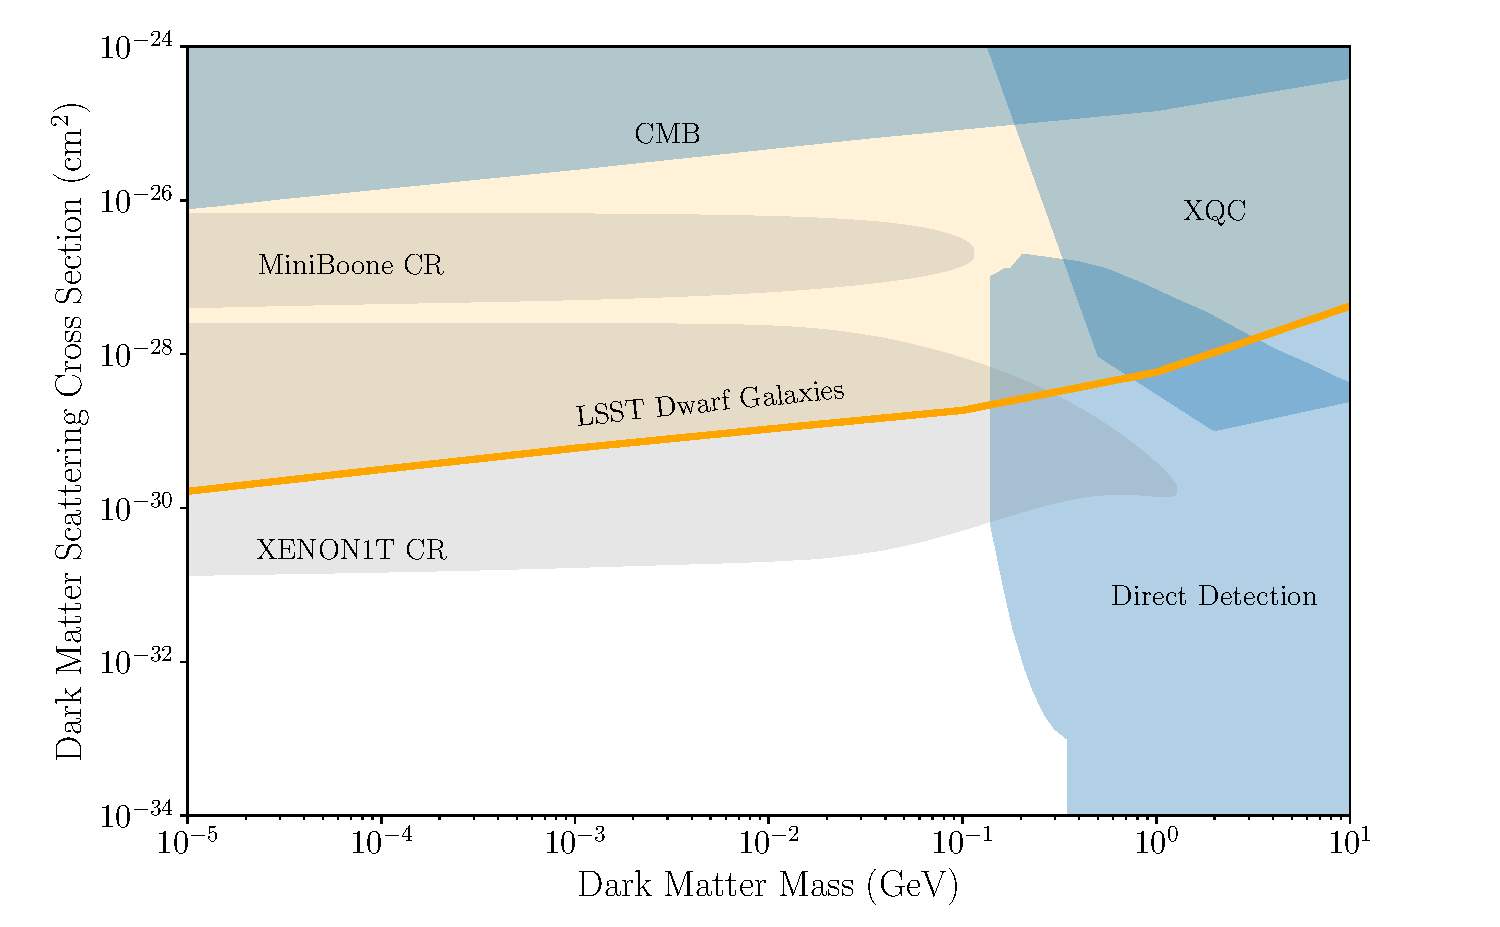
\includegraphics[width=0.75\columnwidth]{bsdm_limits.pdf}
\caption{
Constraints on dark matter-baryon scattering through a velocity-independent, spin-independent contact interaction with protons. 
Existing constraints (shown in blue) include measurements of the CMB power spectrum \citep[CMB;][]{Gluscevic:2017ywp} and constraints from the X-ray Quantum Calorimeter experiment \citep[XQC;][]{0704.0794}. Direct detection constraints include results from CRESST-III \citep{1711.07692}, the CRESST 2017 surface run \citep{1707.06749}, and XENON1T \citep{1705.06655}, as interpreted by \citet[][]{1802.04764}. %\citep{2018PhRvD..97l3013K}.
Additional constraints that include the effects of cosmic-ray heating of dark matter are shown in gray \citep[][]{1810.10543}.
The projected sensitivity of LSST to dark matter-baryon scattering through observations of Milky Way satellite dwarf galaxies is shown in gold.
}
\label{fig:dd}
\end{figure}

The most sensitive direct searches for dark matter seek to detect the scattering of dark matter particles from the local Galactic halo in underground detectors \citep[\eg,][]{1509.08767}. 
They have unprecedented sensitivity to WIMPs with masses above a GeV, but are limited by kinematics when searching for lighter particles. 
New experimental techniques are being explored to directly search for sub-GeV models of dark matter \citep{Battaglieri:2017aum}. 
However, due to atmospheric and terrestrial shielding, most direct dark matter experiments are largely insensitive to dark matter particles with large scattering cross sections. 
Current null results from conventional direct detection experiments motivate broad searches in regions of parameter space that are largely inaccessible to underground experiments. 

%This has motivated a number of experimental tests using astrophysical and cosmological measurements including the X-ray Quantum Calorimeter experiment \citep[XQC;][]{0704.0794} and studies of dark matter-cosmic-ray interactions \citep{Cappiello:2018hsu,1810.10543}.

Cosmological and astrophysical observables are sensitive to the scattering of sub-GeV particles with baryons at any point in cosmic history. 
These observations can constrain the interaction cross section to arbitrarily high values and are not subject to uncertainties in the local astrophysical properties of dark matter particles \citep[\eg,][]{1210.2721,1404.1938}. 
If dark matter particles scatter with baryons, they will transfer momentum between the two cosmological fluids, affecting density fluctuations and suppressing power at small scales. 
This power suppression can be captured by a variety of observables including measurements of the CMB \citep{1311.2937,Gluscevic:2017ywp} and the Lyman-$\alpha$ forest \citep{Xu:2018efh}.
Assuming a velocity-independent, spin-independent contact interaction, cosmological constraints can be directly compared against those from direct detection experiments \citep[\eg,][]{Boddy:2018kfv}.
In \figref{dd}, we compare existing constraints on dark matter-baryon scattering from analyses of the CMB and direct-detection searches.\footnote{We caution the reader that this figure does not include a comprehensive list of current constraints, but rather serves to illustrate the complementarity of cosmological and direct detection probes.} 
To estimate the future sensitivity of LSST, we map the projected WDM constraints presented in \secref{smallest_galaxies} to a dark matter-baryon scattering constraints by matching the characteristic cutoff scale in the matter power spectrum probed by the lowest-mass subhalos LSST can detect via observations of Milky Way satellite galaxies. 
LSST will deliver measurements of observables that trace matter fluctuations on even smaller scales (\eg, stellar stream gaps), which will potentially extend the sensitivity of these astrophysical and cosmological searches even farther beyond the reach of Planck.